\documentclass[12pt]{article}
\usepackage[top=2cm, bottom=3cm, left=1.5cm, right=1.5cm]{geometry}
\usepackage{amsmath,amsthm}
\usepackage{bm}
\usepackage{color}
\usepackage{graphicx}
\usepackage{epstopdf}
\usepackage{enumitem}
\usepackage{amsfonts}
\usepackage{subcaption}
\usepackage{fourier}
\usepackage{ctex}
\begin{document}
\title{平面几何第二次讲座讲义}
\author{赵丰\footnotesize \texttt{616545598@qq.com}\footnote{Copyright: Creative Commons Attribution-Share Alike 4.0 International}}
\maketitle
{\bf 关键词: 圆幂,托勒密定理,根轴}
\begin{enumerate}
\item 
如图\ref{fig:Power_point_simple} 所示,$PT$是圆$O$的切线,$T$为切点,$PMN$是圆$O$的割线,由$\triangle PTM\sim \triangle PTN$得$PT^2=PM\cdot PN$,
同理$PT^2=PA*PB=(PO-PA)\cdot(PO+OB)=PO^2-AO^2$,称$PT^2$为$P$点对圆$O$的幂。

    \begin{figure}[!ht]
    \centering
    \begin{subfigure}[b]{0.53\textwidth}
    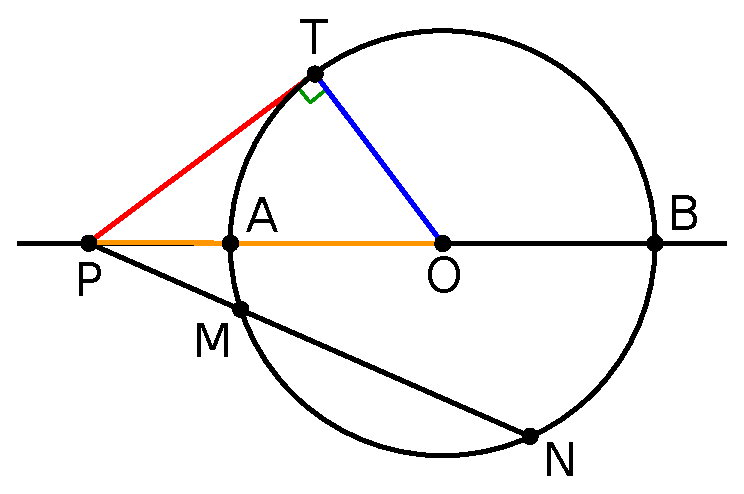
\includegraphics[width=\textwidth]{Power_point_simple.eps}
    \caption{$P$在圆外}\label{fig:Power_point_simple}
    \end{subfigure}~
    \begin{subfigure}[b]{0.37\textwidth}

    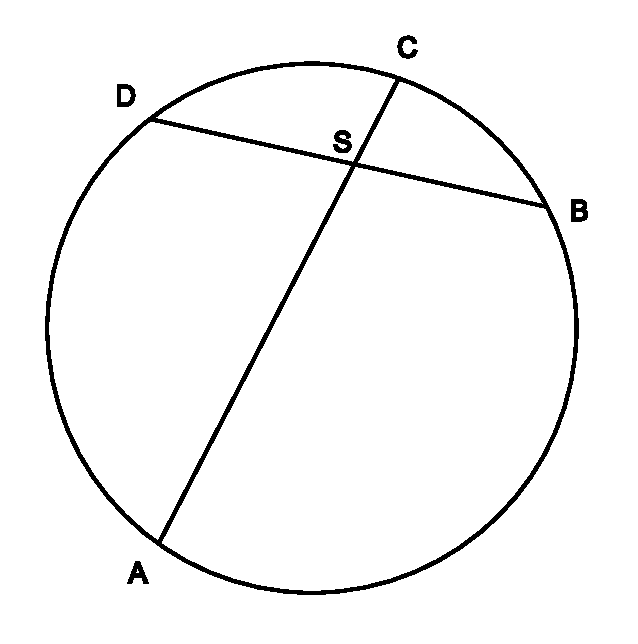
\includegraphics[width=\textwidth]{Chord_theorem.eps}
    \caption{$S$在圆内}\label{fig:Chord_theorem}
    \end{subfigure}
    \end{figure}

如图\ref{fig:Chord_theorem} 所示,当$S$在圆内时,有$AS\cdot SC=BS\cdot SD$\footnote{$S$\textcolor{red}{在圆内时,圆幂是负值,其绝对值等于}$AS\cdot SC$}。
并且有 
\begin{equation}\label{eq:Ptolemy_theorem}
AD\cdot BC+AB\cdot CD = AC\cdot BD
\end{equation}
\eqref{eq:Ptolemy_theorem}式即为托勒密定理。

\textbf{作业}:证明托勒密定理。
\item 
如图\ref{fig:Radical_axis_orthogonal_circles} 所示,$P$到两圆的幂相等,即切线长相等,则$PO_1^2-r_1^2=PO_2^2-r_2^2$,其中$r_1,r_2$分别为$O_1,O_2$的半径。
$PQ\perp O_1O_2$。由勾股定理$PO_1^2-PO_2^2=QO_1^2-QO_2^2\Rightarrow QO_1^2-r_1^2=QO_2^2-r_2^2$,所以$Q$到两圆的幂相等。由$P$的任意性,直线$PO$上所有的点对两圆等幂。称$PQ$为两圆的根轴,根轴垂直于连心线。

    \begin{figure}[!ht]
    \centering
    \begin{subfigure}[b]{0.45\textwidth}
    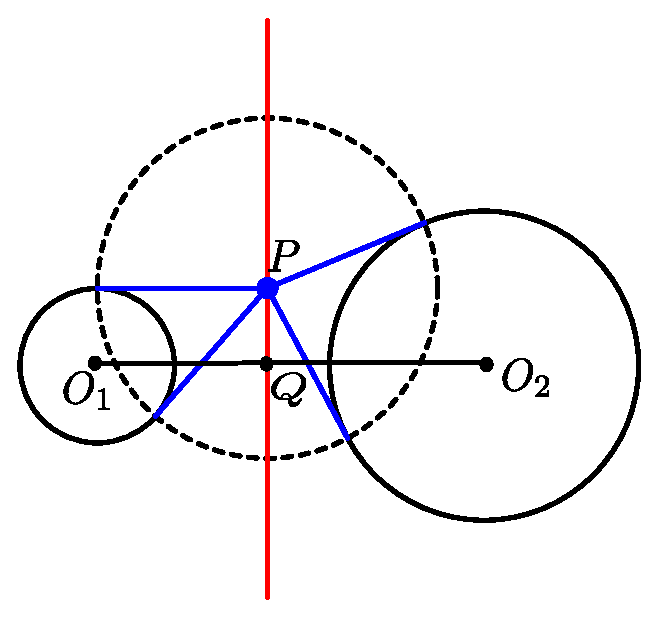
\includegraphics[width=\textwidth]{Radical_axis_orthogonal_circles.eps}
    \caption{两圆不交}\label{fig:Radical_axis_orthogonal_circles}
    \end{subfigure}~
    \begin{subfigure}[b]{0.45\textwidth}
    \includegraphics[width=\textwidth]{Radical_axis_intersecting_circles.eps}
    \caption{两圆相交}\label{fig:Radical_axis_intersecting_circles}
    \end{subfigure}
    \caption{根轴定理示意图}
    \end{figure}

如图\ref{fig:Radical_axis_intersecting_circles} 所示,当两圆相交时,公共弦所在直线即为根轴。

\item 
课堂练习:
    \begin{figure}[!ht]
    \centering
    \begin{subfigure}[b]{0.45\textwidth}
    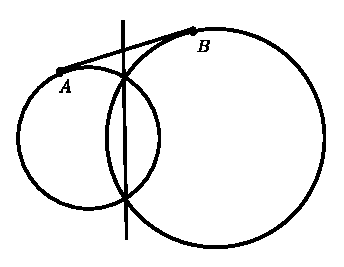
\includegraphics[width=\textwidth]{second_1.eps}
    \caption{}\label{fig:second_1}
    \end{subfigure}~
    \begin{subfigure}[b]{0.45\textwidth}
    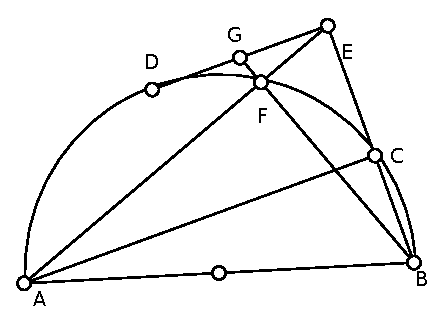
\includegraphics[width=\textwidth]{second_2.eps}
    \caption{}\label{fig:second_2}
    \end{subfigure}
    \caption{}
    \end{figure}
\begin{enumerate}[label=(\alph*)]
\item (圆幂)如图\ref{fig:second_1},$\Gamma_1,\Gamma_2$是两个相交的圆。$AB$是$\Gamma_1,\Gamma_2$的公切线,$A,B$分别是切点。证明两圆的公共弦平分$AB$。


\item \textbf{作业}:(综合)如图\ref{fig:second_2},设 $C$是直径为$AB$的半圆上的一点,$D$是弧$AC$的中点。过$D$作$BC$的垂线,垂足为$E$,$F$是$AE$和半圆的交点。证明$BF$的延长线平分线段$DE$。(提示:设圆心为$O$,连接$DO$交$AE$于$J$,交$AC$于$H$,说明$DECH$是长方形,由此推出$DJ=\frac{1}{2}EC,结合\triangle DJE\sim \triangle GEB \Rightarrow \frac{DJ}{GE}=\frac{DE}{EB}$,利用$DHCE$\textcolor{red}{是矩形说明}$DE$\textcolor{red}{是切线},$DE^2=GE\cdot EB \Rightarrow DE=2GE$)

    \begin{figure}[!ht]
    \centering
    \begin{subfigure}[b]{0.45\textwidth}
    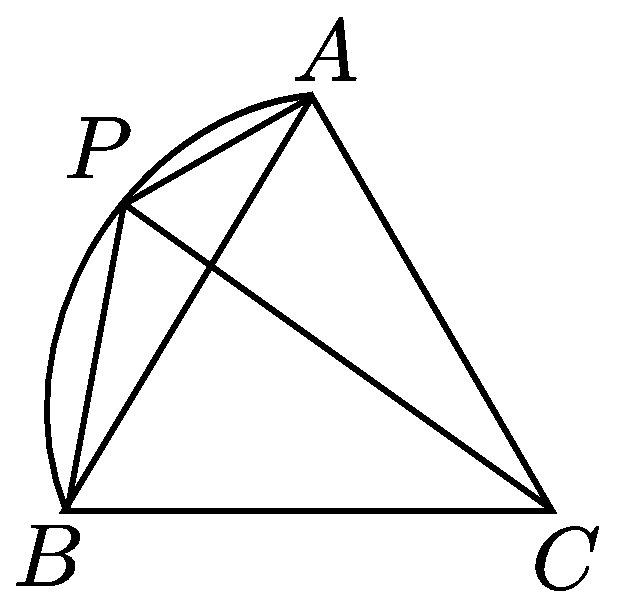
\includegraphics[width=\textwidth]{second_3.eps}
    \caption{}\label{fig:second_3}
    \end{subfigure}~
    \begin{subfigure}[b]{0.45\textwidth}
    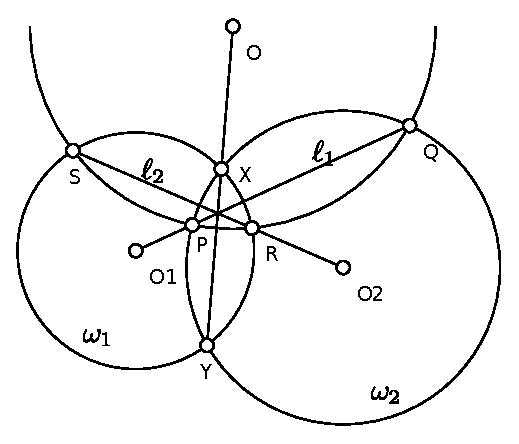
\includegraphics[width=\textwidth]{second_4.eps}
    \caption{}\label{fig:second_4}
    \end{subfigure}
    \caption{}
    \end{figure}

\item
(托勒密定理)如图\ref{fig:second_3},$\triangle ABC$ 是等边三角形,$P$是$\triangle ABC$ 外接圆弧上劣弧$AB$上一点,证明$PC=PA+PB$。能否用全等三角形证明?

\item (根轴)
如图\ref{fig:second_4},圆$\omega_1,\omega_2$相交于$X,Y$,直线$\ell_1$过$\omega_1$的圆心$O_1$交$\omega_2$于$P,Q$两点,
直线$\ell_2$过$\omega_2$的圆心$O_2$交$\omega_1$于$R,S$两点。已知$P,Q,R,S$四点共圆,圆心为$O$。求证:圆心$O$在直线$XY$上。
(提示:设$P,Q,R,S$四点圆为$\omega$,$O_1$在$\omega,\omega_2$两圆的根轴上,$O_1$对$\omega$的幂等于$O_1$对$\omega_2$的幂,同理
$O_2$对$\omega$的幂等于$O_2$对$\omega_1$的幂,利用这两个等式可以推出$O$对$\omega_1$的幂等于$O$对$\omega_2$的幂)
\end{enumerate}
\item \textbf{作业}
\begin{enumerate}[label=(\alph*)]
\item (倒角)如图\ref{fig:second_5}所示,$A,B,C,D$是平面上四个不同的点,$AC$和$BD$不平行。$AC$和$BD$交于$E$。
$\triangle ABE$的外接圆与$\triangle CDE$的外接圆 相交于点$F$。证明$\triangle AFC \sim \triangle BFD$。

    \begin{figure}[!ht]
    \centering
    \begin{subfigure}[b]{0.5\textwidth}
    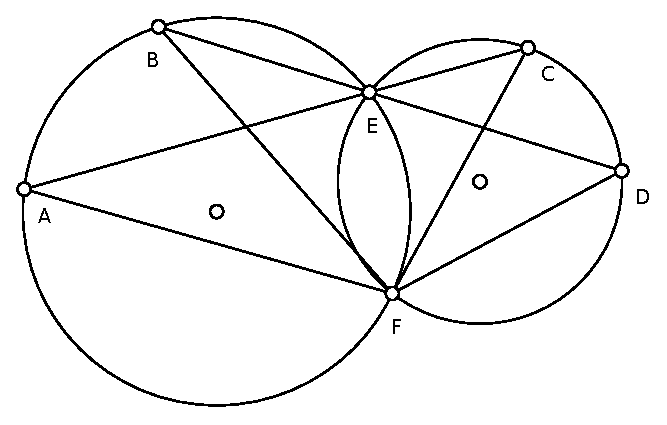
\includegraphics[width=\textwidth]{second_5.eps}
    \caption{}\label{fig:second_5}
    \end{subfigure}~
    \begin{subfigure}[b]{0.4\textwidth}
    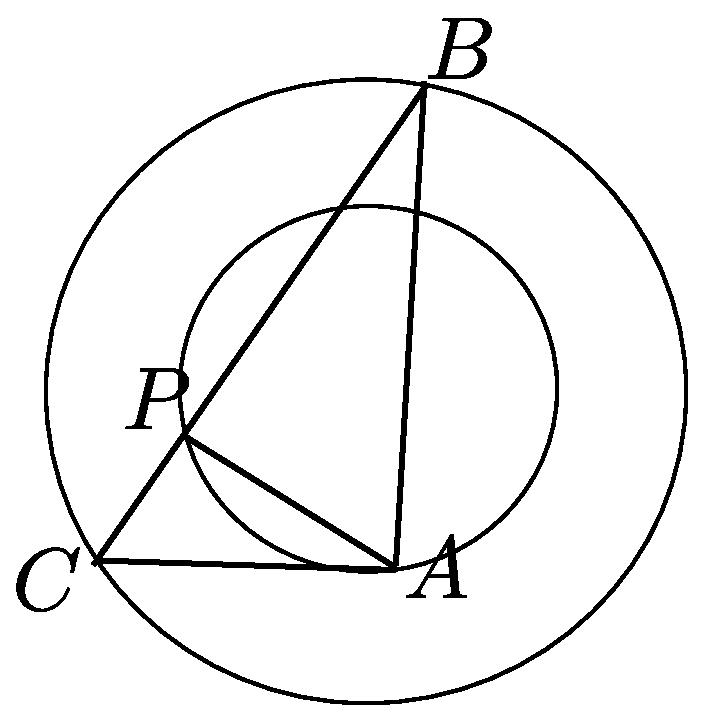
\includegraphics[width=\textwidth]{second_6.eps}
    \caption{}\label{fig:second_6}
    \end{subfigure}
    \caption{}
    \end{figure}
\item (圆幂)如图\ref{fig:second_6}所示,考虑两个同心圆,半径分别为$R$和$r(R>r)$。$P$在小圆圆弧上,$B$在大圆圆弧上,$BP$交大圆圆弧于$C$。过$P$作$BP$的垂线交小圆圆弧于$A$。证明:$BC^2+CA^2+AB^2=6R^2+2r^2$ (提示:设$BC$交小圆圆弧于$Q$,$BQ=CP,AQ=2r,CP\cdot PB=R^2-r^2$,利用圆幂、勾股定理计算化简)
\end{enumerate}
\end{enumerate}

\end{document}
